\chapter{Hardwarové komponenty}

\section{Sběrnice}

Sběrnice představuje do jisté míry nervový systém celého emulátoru, neboť nejen propojuje hlavní 
hardwarové komponenty, ale musí se také starat o jejich paměťovou správu. 
Díky tomu faktoru, sběrnice v emulátoru vytváří všechny komponenty a řeší jejich vzájemné závislosti.

Jelikož komponenty mohou být vzájemně sdíleny, bylo nutné zvolit vhodnou 
strukturu pro správu jednotlivých objektů. Pro tyto účely jsem se rozhodl použít \textit{shared\_ptr} ze 
standardní knihovny \textit{C++}. Nejenže paměť bude spravována automaticky, ale lze velice jednoduše vytvořit duplicitní reference na tentýž objekt.

\begin{figure}[hbt]
\centering
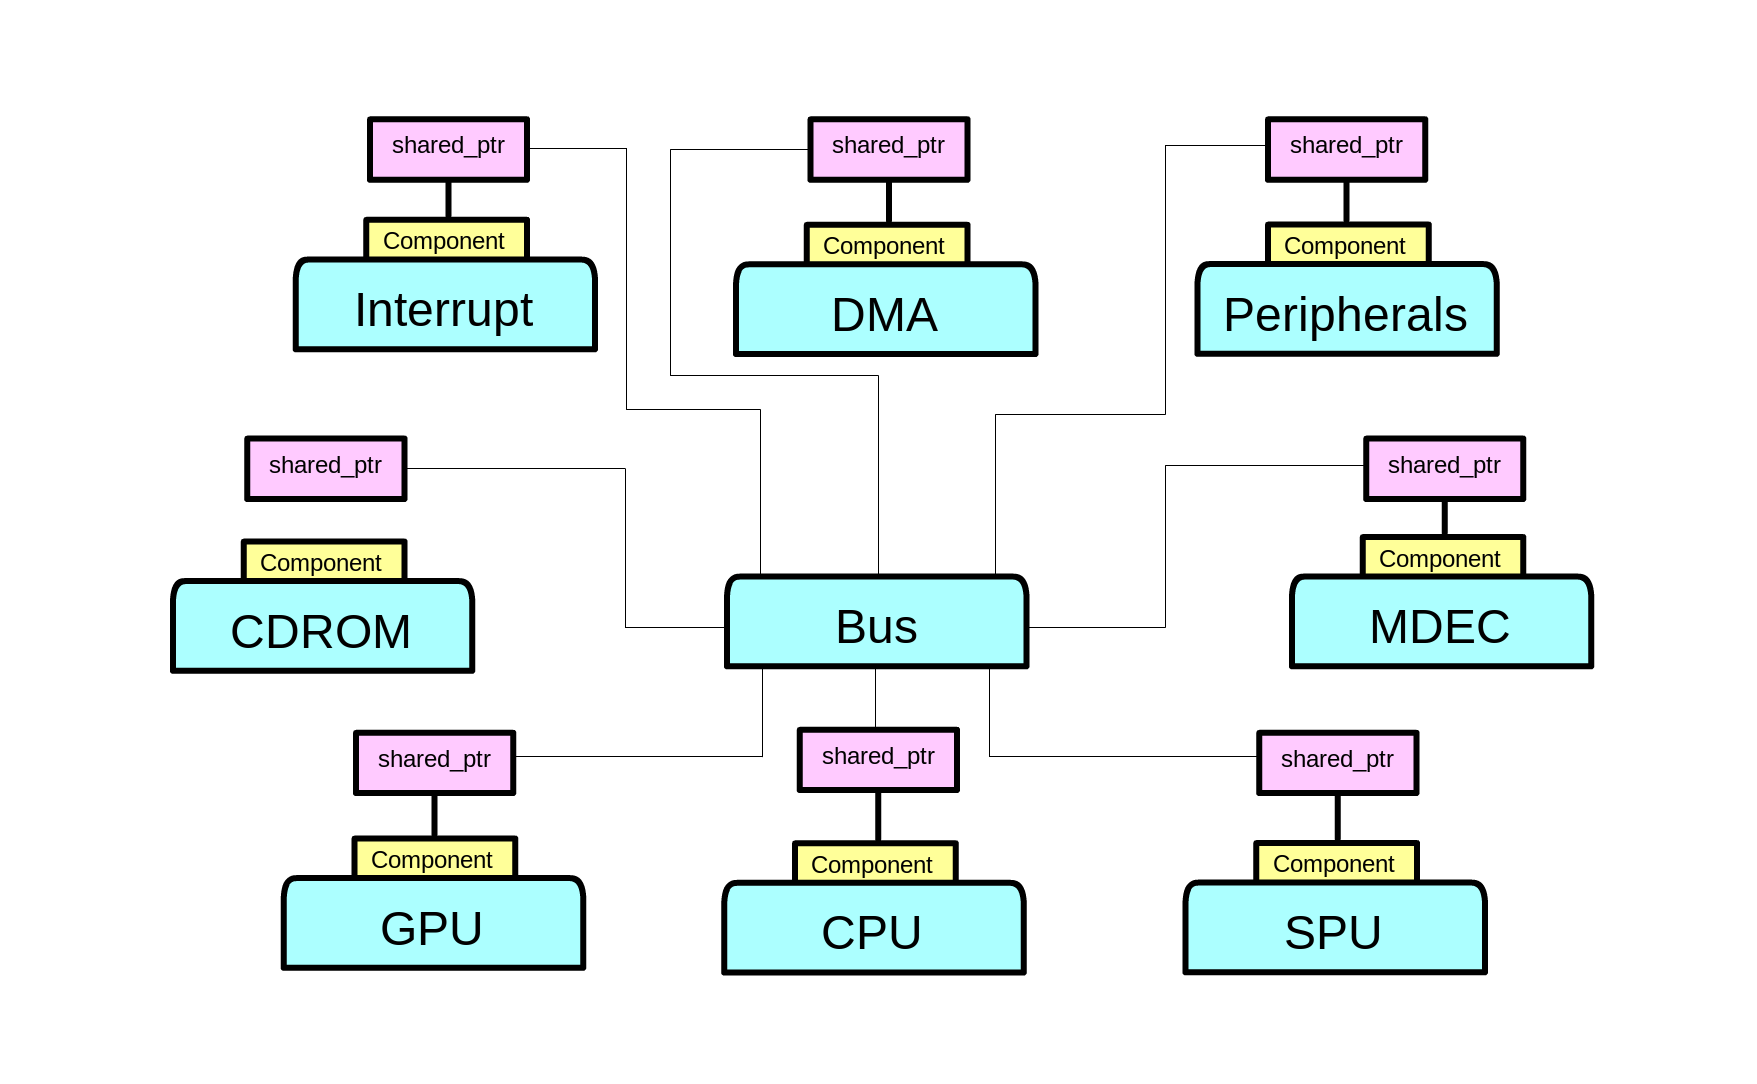
\includegraphics[width=0.8\textwidth]{obrazky-figures/bus-ownage.png}
\caption{Sběrnice pomocí \textit{shared\_ptr} struktury může vlastnit jednotlivé komponenty, ale také umožňuje sdílení mezi těmito komponentami.}
\label{bus-ownage}
\end{figure}

Další zodpovědností sběrnice je správné distribuce čtení a zápisů jednotlivým komponentám. 
Všechny tyto paměťové operace závisejí na \textit{Memory-mapped I/O}. \textit{Memory-mapped I/O} mapuje 
lineární 32-bitový paměťový prostor na segmenty, skrz které může sběrnice ovládat jednotlivé komponenty\footnote{Paměťová mapa PlayStation\cite{PSXSpec} \url{https://psx-spx.consoledev.net/iomap/}}.

\begin{table}[htbp]
\caption{Paměťová mapa}
\begin{center}
\begin{tabular}{ |c|c|r| }
 \hline
 \textbf{Název} & \textbf{Lokace} & \textbf{Velikost} \\
 \hline
 RAM & 0x00000000 & 2 MiB \\
 Expansion & 0x1F000000 & 1 MiB \\
 Scratchpad & 0x1F800000 & 1 KiB \\
 Ovladač paměti & 0x1F801000 & 36 B \\
 Periférie & 0x1F801040 & 16 B \\
 Serial & 0x1F801050 & 16 B \\
 Ovladač RAM & 0x1F801060 & 4 B \\
 Ovladač přerušení & 0x1F801070 & 8 B \\
 DMA & 0x1F801080 & 128 B \\
 DotClock Časovač & 0x1F801100 & 16 B \\
 HBlank Časovač & 0x1F801110 & 16 B \\
 SystemClock/8 Časovač & 0x1F801120 & 16 B \\
 CDROM & 0x1F801800 & 4 B \\
 GPU & 0x1F801810 & 8 B \\
 MDEC & 0x1F801820 & 8 B \\
 SPU & 0x1F801C00 & 1 KiB \\
 I/O porty & 0x1F802000 & 8 KiB \\
 BIOS & 0x1FC00000 & 512 KiB \\
 Ovladač cache & 0x1FFE0130 & 4 B \\
 \hline
\end{tabular}
\end{center}
\end{table}

Jelikož sběrnice má 32-bitovou šířku, mohlo by se zdát, že stačí pouze na základě paměťové mapy vzít danou 
adresu a rozdistribuovat ji příslušné komponentě. Nicméně sběrnice tohoto systému má 2 zvláštnosti: 
Správa virtuální paměti a přímý zápis do vyrovnávací paměti instrukcí.

\subsection{Virtuální paměť}

Jak bylo naznačeno, \textit{PlayStation} je do jisté míry zjednodušená verze 
deskového počítače a existují určité artefakty, které jsou pozůstatky plné funkčnosti deskového počítače. 
Jedním z takovýchto artefaktů je virtuální paměť. I přesto, že procesor má 
podporu \textit{Translation Lookaside Bufferu (TLB)} pro efektivní správu virtuální paměti, \textit{PlayStation} jej vůbec nevyužívá a všechny přístupy do paměti jsou v zásadě absolutní.
To, co zůstalo z virtualizace paměti, je maskování všech adres které přijdou na sběrnici a na základě velikosti zapisovaných či čtených dat probíhá maskování odlišně.
Nejdříve se u každého přístupu zahodí vrchní 3 bity. 
Poté u půl-slova (16 bitů) se zahodí spodní 1 bit a u slova (32 bitů) se zahodí spodní 2 bity. 
Zahození spodních bitů souvisí se zarovnáním do paměti\footnote{Přístup do paměti\cite{PSXSpec} \url{https://psx-spx.consoledev.net/memorymap/}}.

\subsection{Vyrovnávací paměť instrukcí}

Druhá zvláštnost, na kterou je třeba myslet při distribuci čtení a zápisu, je vyrovnávací paměť instrukcí uvnitř \textit{CPU}. 
Tato vyrovnávací paměť slouží pro rychlé získávání instrukcí z hlavní paměti a teoreticky by nikdy 
neměla nastat situace, kdy ve vyrovnávací paměti bude něco jiného, než co je obsaženo v hlavní paměti. 
Ovšem to není u tohoto systému vždy pravda.

\textit{CPU} má speciální stav, který se dá programaticky nastavit a který takzvaně izoluje vyrovnávací paměť instrukcí. 
Pokud \textit{CPU} se nachází v tomto stavu, pak každé čtení za účelem získat instrukci (\textit{fetch} fáze \textit{CPU}) 
nikdy nebude putovat do hlavní paměti, ale do této vyrovnávací paměti a \textbf{každý} zápis bude modifikovat vyrovnávací paměť místo hlavní paměti. 
\textit{CPU} tedy jinými slovy poskytuje přímý přístup do této vyrovnávací paměti.
Pokud toto není správně ošetřeno a simulováno, \textit{PlayStation} nebude schopen nastartovat\footnote{Koprocesor 0, registr 12, bit 16\cite{PSXSpec} \url{https://psx-spx.consoledev.net/cpuspecifications/\#cop0r12-sr-system-status-register-rw}}.

\subsection{Časování}

Každá hardwarová komponenta pracuje v reálném čase paralelně a nezávisle. Situaci dále zhoršuje fakt, že každá komponenta má odlišnou frekvenci hodin\footnote{Časování\cite{PSXSpec} \url{https://psx-spx.consoledev.net/timers/}, \url{https://psx-spx.consoledev.net/graphicsprocessingunitgpu/\#gpu-timings}}.

\begin{itemize}
    \label{Rychlost hodin komponent}
    \item{\textbf{CPU} - 33.868800 MHz}
    \item{\textbf{GPU} - 53.222400 MHz}
    \item{\textbf{SPU} - 44.100 KHz}
    \item{\textbf{DotClock Timer} - 4.980705 MHz (Průměr)}
    \item{\textbf{HBlank Timer} - 9923 Hz (NTSC), 9943 Hz (PAL)}
    \item{\textbf{System Clock/8 Timer} - 4.233600 MHz}
\end{itemize}

Tento problém je řešen tak, že emulátor simuluje každou komponentu sekvenčně a zvlášť v malých kvantech. 
Množství hodinových cyklů alokovaných pro danou komponentu reflektuje předchozí list hodnot. 
Tato simulace může způsobit časovou dilataci mezi jednotlivými komponentami a vést k narušení jejich synchronizace. 
Při volbě časového kvanta ho nesmíme zvolit příliš malé, protože by došlo k nesprávnému zaokrouhlení na základě časovací tabulky a nepřesnost časování by byla větší. 
Zároveň však kvantum nesmíme zvolit příliš velké, protože by se komponenty nemusely dostat včas ke slovu. 
Dvě komponenty, pro které je synchronizace nejdůležitější, jsou \textit{CPU} a \textit{GPU}. 
Přičemž \textit{GPU} je o $\frac{11}{7}$ rychlejší, zvolil jsem tedy časovou konstantu $301$, protože výsledek formule $301\times\frac{11}{7}=473$ je celé číslo a není
třeba řešit zlomkovou část časování.

\section{CPU}

Pokud je sběrnice nervovým systémem, pak \textit{CPU} je mozkem \textit{PlayStation} systému. Jde
o \textit{MIPS R3000A} 32-bitový \textit{RISC} procesor TODO: source. Jeho architektura je založena na \textit{MIPS I} redukované instrukční sadě.
\textit{CPU} má celkem 5 stavů, ve kterých se může nacházet a které provádí v nepřetržité smyčce:

\begin{itemize}
    \item{\textbf{Fetch (IF)} fáze - získání následující instrukce z paměti \textit{RAM}.}
    \item{\textbf{Decode (ID)} fáze - dekódování instrukce a zjištění následující operace.}
    \item{\textbf{Execute (EX)} fáze - \textit{CPU} provede dekódovanou instrukci (aritmetickou či logickou operaci).}
    \item{\textbf{Memory Access (MEM)} fáze - pokud instrukce přistupuje do paměti, data jsou pomocí sběrnice přečtena či zapsána do paměti \textit{RAM}.}
    \item{\textbf{Write Back(WB)} fáze - Výsledek instrukce je zapsán do souboru registrů.}
\end{itemize}

\subsection{Vnitřní stav \textit{CPU}}

Pro ukládání mezivýsledků a pro obecné zpracování logiky, \textit{CPU} obsahuje celkem \textbf{32} 32-bitových registrů, plus \textbf{2} 32-bitové registry, které
jsou specializované pro práci s násobícími a dělícími instrukcemi\cite{MIPSSpec}. 
\textit{Nultý} registr je speciální tím, že při čtení vrací vždy nulu a jakýkoliv zápis do něj je ignorován.

\subsection{Zpoždění načítání hodnot}

\textit{MIPS R3000A}, jako každý \textit{RISC} procesor, vykazuje zvláštní jev při načítání hodnot do registrů.
Pokud se snažíme načíst hodnotu z paměti \textit{RAM} do procesoru, zpoždění způsobené načítáním hodnoty má za následek
opožděné nastavení registru na přečtenou hodnotu o jeden procesorový takt\cite{MIPSSpec}. 
Toto je způsobeno samotným návrhem \textit{RISC} architektury a je nutné tuto situaci ošetřit. 

V emulátoru je tento fenomén simulován pomocí dvou registrových přihrádek, které fungují jako fronta.
Kdykoliv \textit{CPU} chce přečíst hodnotu z paměti \textit{RAM}, místo přímého nastavení registru,
přečtená hodnota spolu s indexem výsledného registru v prvním taktu je vložena do fronty a po druhém taktu se 
zmodifikuje registrové pole.

Je nutné také pamatovat na situaci, kdy ve frontě je připravená hodnota, ale mezitím přijde jiná instrukce, 
která stejný registr modifikuje. V takovém případě je nutné frontu vyčistit, aby se výsledný registr špatně
nezmodifikoval.

\subsection{Zpoždění skoku}

Podobně jako opožděné načítání hodnot do registru, design 5 stupňové architektury má na svědomí ještě jeden problém.
Tento artefakt se vyskytuje u všech skokových instrukcí a má za následek, že bez ohledu na to, zda-li se skočí nebo ne 
(v případě podmíněných skoků), následující instrukce po skoku se vždy provede\cite{MIPSSpec}.

To je způsobeno tím, že následující instrukce je již načtena a dekódována uvnitř \textit{CPU}. 
Kompilátory té doby byly dobře seznámeny s tímto fenoménem a ve většině případů vyplnily instrukci za skokem prázdnou instrukcí. 
Z tohoto důvodu je každý skok v emulátoru zpožděn o jeden takt.

\subsection{Instrukční sada}

\begin{figure}[hbt]
	\centering
	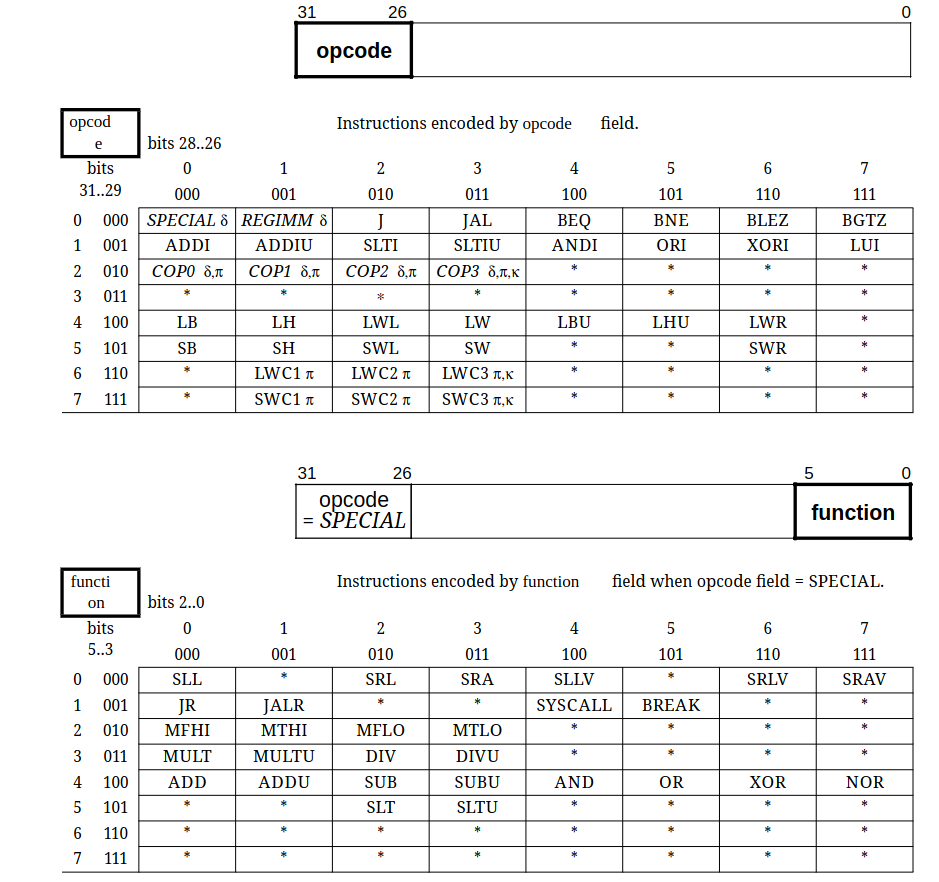
\includegraphics[width=0.8\textwidth]{obrazky-figures/instruction-map.png}
	\caption{Kompletní mapa všech \textbf{69} instrukcí podle specifikace\cite{MIPSInsSpec}.}
	\label{instruction-map}
\end{figure}

\begin{figure}[hbt]
	\centering
	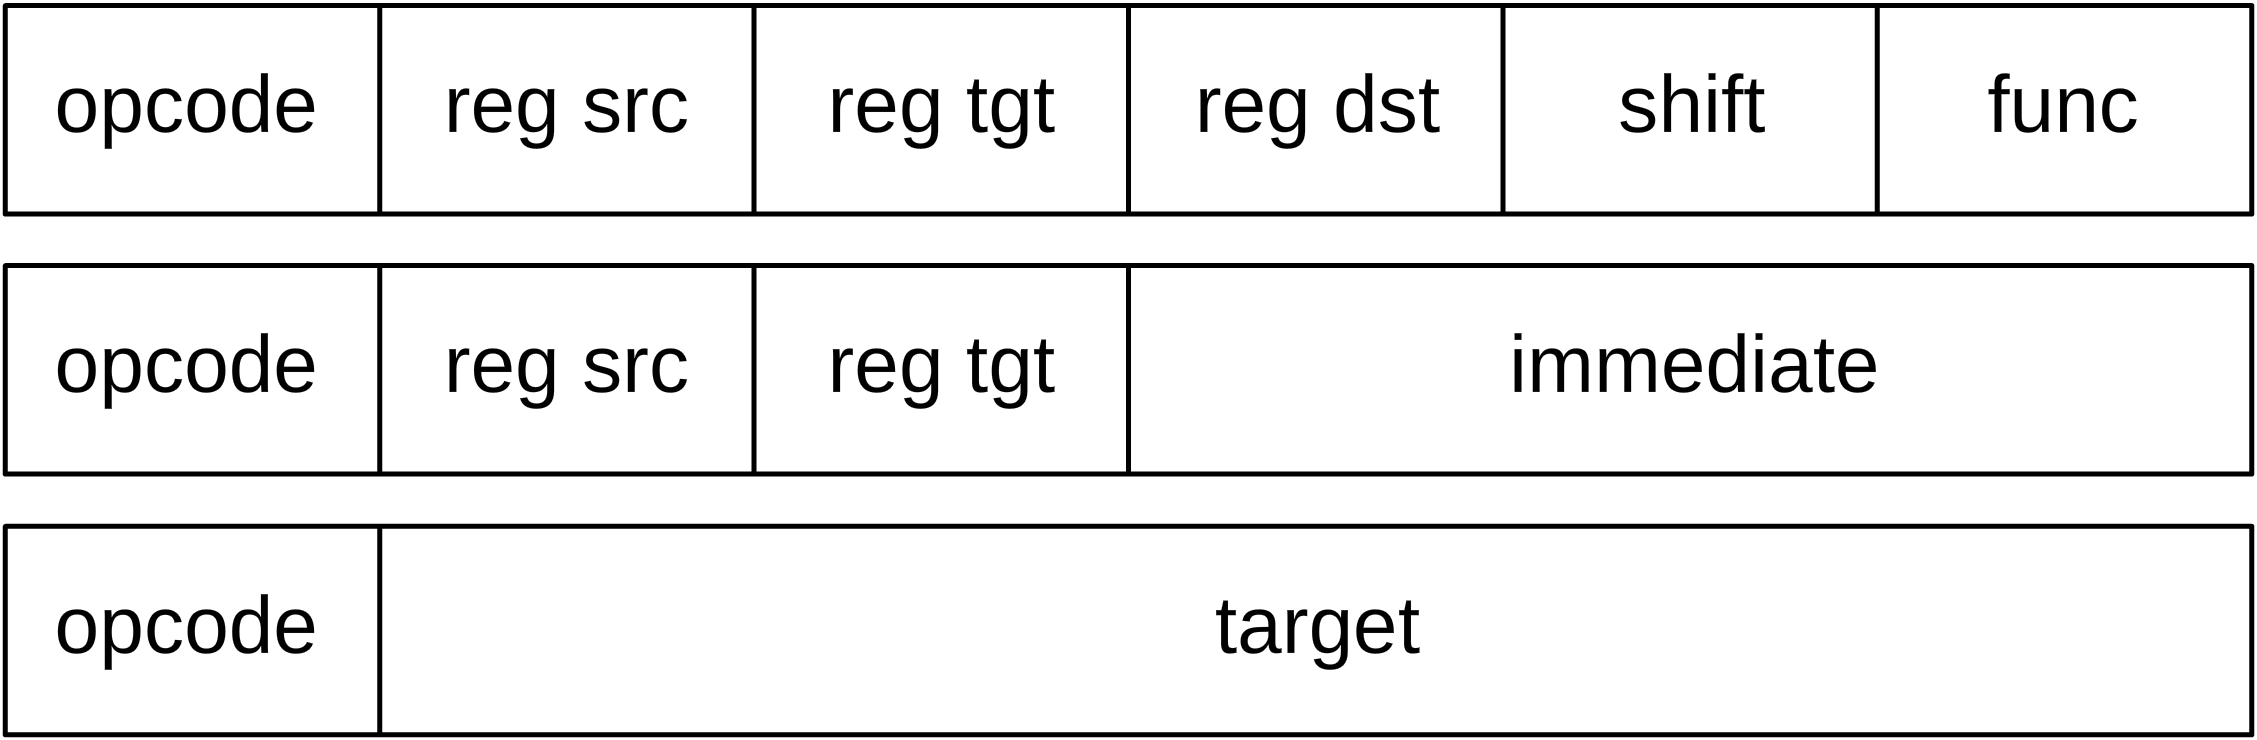
\includegraphics[width=0.8\textwidth]{obrazky-figures/instruction.png}
	\caption{\textit{MIPS} má celkem 3 způsoby, jak zakódovat instrukci do 32 bitů.}
	\label{instruction}
\end{figure}

Instrukční sada \textit{CPU}, založená na architektuře \textit{MIPS I}, obsahuje relativně malý počet instrukcí. 
Tato sada zahrnuje \textit{40} základních instrukcí a \textit{29} rozšířených instrukcí, což dohromady činí \textbf{69} instrukcí celkem\cite{MIPSInsSpec}. 
Tyto instrukce jsou navrženy tak, aby každá z nich zabírala jeden procesorový takt, čímž je udržována neustále plněná 5-ti úrovňová linka. 
Díky této filozofii mají instrukce velmi málo zodpovědností a jsou v podstatě velmi jednoduché.

Aby se předešlo složitému dekódování instrukcí, jak tomu například je u architektury \textit{x64}, 
kde každá instrukce může mít různou délku, \textit{MIPS I} definuje každou instrukci jako 32-bitové slovo. 
Horních 6 bitů pak definuje kódování specifické instrukce. I přesto lze každou instrukci rozdělit do zhruba tří tříd [\ref{instruction}].

\subsection{Koprocesory}

\textit{MIPS R3000A} ve své instrukční sadě má podporu pro celkem 4 různé koprocesory, avšak \textit{PlayStation} využívá pouze 2 z nich\footnote{CPU specifikace\cite{PSXSpec} \url{https://psx-spx.consoledev.net/cpuspecifications/}}. 
Koprocesorové instrukce jsou všestranné a lze za ně substituovat jakýkoliv čip, kromě \textbf{koprocesoru 1}, který je dedikován pro práci s čísly s plovoucí desetinnou čárkou (není přítomen v \textit{PlayStation} konzoli)\cite{MIPSInsSpec}.

\textbf{Koprocesor 0} slouží ke správě výjimek a přerušení. 
Koprocesor obsahuje nejen informace o typu výjimky nebo tom, kdo způsobil přerušení, ale také logiku pro zpracování výjimky. 
Procesor při vyhození výjimky uloží současný stav a jeho kontrolní tok je přenesen na rutinu, která se stará o obsluhu výjimky.

\textbf{Koprocesor 2} pak zpřístupňuje komponentu \textit{Geometry Transformation Engine (GTE)}, což je hardware specializovaný pro rychlou práci s lineární algebrou. 
Tento koprocesor pracuje s dvěma základními datovými primitivy: 3D vektory (16/32-bitový atom) a 3x3 matice (16/32-bitový atom). 
Vektory mohou být interpretovány jako body v prostoru nebo jako barvy a pro každý typ má \textit{GTE} dedikované příkazy. 
Funkce \textit{GTE} jsou velmi všestranné, zahrnují rychlé násobení matice s vektorem, normalizaci barev nebo vektoru a dokonce i interpolaci. 
Tento koprocesor je nepochybně klíčový pro rychlé zpracování geometrie ve hře a rychlé vykreslení 3D scény.

\section{GPU}

Grafická jednotka systému je speciálně navržený čip pro hardwarovou podporu rasterizace geometrických primitiv\footnote{GPU specifikace\cite{PSXSpec} \url{https://psx-spx.consoledev.net/graphicsprocessingunitgpu/}}.
\textit{GPU} pracuje na frekvenci 53.222400 MHz, což znamená, že je o $\frac{11}{7}$ rychlejší než frekvence \textit{CPU}. Všechna komunikace s \textit{GPU} probíhá přes
čtyři registry:

\begin{itemize}
\item{\textbf{GP0} (pouze zápis) - registr pro odesílání rasterizačních příkazů a posílání geometrických dat. Různé grafické příkazy mohou mít různou délku (počet zapsaných 32-bitových slov).}
\item{\textbf{GP1} (pouze zápis) - registr pro modifikaci stavu \textit{GPU} (například: reset, nastavení rasterizačního okna či potvrzení přerušení).}
\item{\textbf{GPUREAD} (pouze čtení) - registr pro čtení \textit{VRAM} paměti nebo pro čtení speciálních registrů.}
\item{\textbf{GPUSTAT} (pouze čtení) - registr pro čtení celkového stavu \textit{GPU}.}
\end{itemize}

\subsection{VRAM}

\textit{GPU} má také vlastní paměť nazývanou \textit{Video RAM (VRAM)}. Paměť je rozdělena do 512 řádků o 1024 16bitových slovech.
Celková kapacita paměti \textit{VRAM} je tedy $1024 \times 512 \times 2 = 1048576 B = 1 MiB$\footnote{GPU VRAM\cite{PSXSpec} \url{https://psx-spx.consoledev.net/graphicsprocessingunitgpu/\#gpu-video-memory-vram}}. 
\textit{VRAM} paměť slouží pouze k ukládání textur, palet pro
indexované textury a výsledného \textit{framebufferu}. Jakákoli data o kreslených primitivech (pozice vrcholů či texturovacích souřadnicích)
musí být předána přes registr \textbf{GP0}. I přesto, že \textit{GPU} má různé módy týkající se barevné hloubky (24 bitů a 15 bitů),
výsledný framebuffer musí mít formát 15bitové barvy.

\subsection{Geometrická primitiva}

\textit{GPU} dokáže vykreslit 3 geometrická primitiva:

\begin{itemize}
    \item{Osově zarovnaný obdélník}
    \item{Čára/Polyčára}
    \item{Trojúhelník/Čtyřúhelník}
\end{itemize}

Všechna tato primitiva lze kreslit pomocí \textbf{GP0} registru\footnote{GPU GP0 registr\cite{PSXSpec} \url{https://psx-spx.consoledev.net/graphicsprocessingunitgpu/\#gpu-other-commands}}, 
přičemž je nutné zapsat správný počet argumentů do tohoto registru.
Počet argumentů daného primitiva závisí především na různých vlastnostech daného primitiva. Ačkoliv ne všechny primitiva mohou mít
všechny vlastnosti, \textit{GPU} dokáže rasterizovat jednotlivá primitiva následujícími způsoby:

\begin{itemize}
    \item{\textbf{Texturovací koordináty} - Primitivum má k sobě přiřazenou texturu a každý vrchol má asociované texturovací koordináty.}
    \item{\textbf{Průhlednost} - Na základě předchozího obsahu ve \textit{VRAM} paměti, \textit{GPU} dokáže mixovat barvy ve čtyřech různých módech\footnote{GPU Semi-transparency\cite{PSXSpec} \url{https://psx-spx.consoledev.net/graphicsprocessingunitgpu/\#semi-transparency}}:
        \begin{itemize}
            \item{\textit{half-each} - $result = \frac{background + source}{2}$}
            \item{\textit{additive} - $result = background + source$}
            \item{\textit{subtractive} - $result = background - source$}
            \item{\textit{$\frac{additive}{4}$} - $result = background + \frac{source}{4}$}
        \end{itemize}
    }
    \item{\textbf{Gouraudovo stínování} - Tento atribut je svým názvem trochu zavádějící, neboť gouraudovo stínování souvisí spíše s výpočtem osvětlení. V tomto případě ovšem jde pouze zapnutí interpolace atributů mezi vrcholy primitiva.}
\end{itemize}

\subsection{Barvy}

Jak bylo zmíněno, \textit{GPU} dokáže pracovat s 24-bitovými barvami, které obsahují 3 základní barevné komponenty (červená, zelená a modrá). 
Každému z těchto komponent je alokováno 8 bitů a poté dokáže pracovat s 15-bitovými barvami, kde každé komponentě je přiřazeno pouze 5 bitů.

Ovšem paměť \textit{VRAM} je rozdělena do 16-bitových slov. Je tedy nutné tyto barevné formáty správně mapovat do výsledné 16-bitové barvy. 
15-bitová barva se pouze zkopíruje do paměti \textit{VRAM}, přičemž 24-bitová barva je za pomocí techniky \textit{dithering}\footnote{GPU dithering\cite{PSXSpec} \url{https://psx-spx.consoledev.net/graphicsprocessingunitgpu/\#24bit-rgb-to-15bit-rgb-dithering-enabled-in-texpage-attribute}} rozdistribuována do kreslícího okolí. 
Paměť \textit{VRAM} v každém fragmentu také ukládá extra 1 bit, který figuruje jako kreslící maska. 
Pokud je nejvyšší bit v 16-bitové barvě nastaven na 1, pak tento fragment bude ignorován a nic se do něj nevykreslí.

\subsection{Rasterizace primitiv}

U každého ze 3 geometrických primitiv, které \textit{GPU} dokáže vykreslit, je nutno zvolit správný algoritmus pro jeho rasterizaci.
U rasterizace osově zarovnaného obdélníku stačí zjistit maximum a minimum ve 2D prostoru. Tento omezený prostor může být následně vyplněn.

Rasterizace čáry vyžaduje sofistikovanější přístup, a to \textbf{Digital Differential Analyzer (DDA) algoritmus}\footnote{DDA algoritmus \url{https://en.wikipedia.org/wiki/Digital_differential_analyzer_(graphics_algorithm)}}, 
který na základě výpočtu sklonu čáry dokáže vyplnit fragmenty mezi dvěma body ve 2D prostoru.

Trojúhelníková rasterizace se řadí mezi vyplňovací rasterizační algoritmy. 
Pro jeho implementaci jsem zvolil efektivní \textbf{Pinedův algoritmus}\cite{PinedaAlgorithm}. 
Jeho podstata závisí na rozdělení jednotlivých hran trojúhelníku na poloroviny a u každého fragmentu zjišťovat jeho 
polohu v závislosti na všech polorovinách daného trojúhelníku.

\subsection{Zvýšení rozlišení}

Zvýšení rozlišení se týká především \textit{GPU} a rasterizace jednotlivých primitiv. 
\textit{GPU} ve svém interním stavu ukládá mimo jiné meze \textit{framebufferu}. 
Tyto meze pak figuruji při rasterizaci, kde jakýkoliv pokus kreslit mimo tyto meze bude ignorován. 
Zároveň tyto meze určují, odkud ve \textit{VRAM} paměti se budou brát data pro zasílání 
do \textit{CRT} monitoru.

Pro tyto účely je nutné spravovat zvláštní \textit{framebuffer}, který podle nastavení 
bude mít násobek velikosti současného reálného \textit{framebufferu} uvnitř \textit{GPU}. 
Při každé modifikaci mezí reálného \textit{framebufferu} je nutné zvláštní \textit{framebuffer} 
zničit, zrekonstruovat a znovu spočítat jeho velikost.

Rasterizaci primitiv je pak nutné zachytit a správně přepočítat jejich pozice, stejně jako 
upravit jejich omezující vlastnosti. Největší potíž však bude při adresaci textur a jejich palet. 
Při každém zápisu textury a indexu barvy je nutné koordináty přemapovat do zvláštního \textit{framebufferu}.

\section{DMA}

Jelikož \textit{CPU} má hodinovou rychlost 33.8688 MHz, jakýkoliv přenos dat je nesmírně pomalý. 
Tento fakt je pouze umocněn v situaci, kdy program chce přenést data z paměti \textit{RAM} do jiné hardwarové komponenty. 
Pokud bychom měli jednoduchou smyčku pro kopírování dat s prokládanou inkrementací indexu do paměti (abychom vyplnili zpoždění čtení z paměti \textit{RAM}),
dostaneme 4 instrukce pro kopírování a 3 instrukce pro správu cyklu [\ref{slow-copy}].

\begin{figure}[hbt]
	\centering
	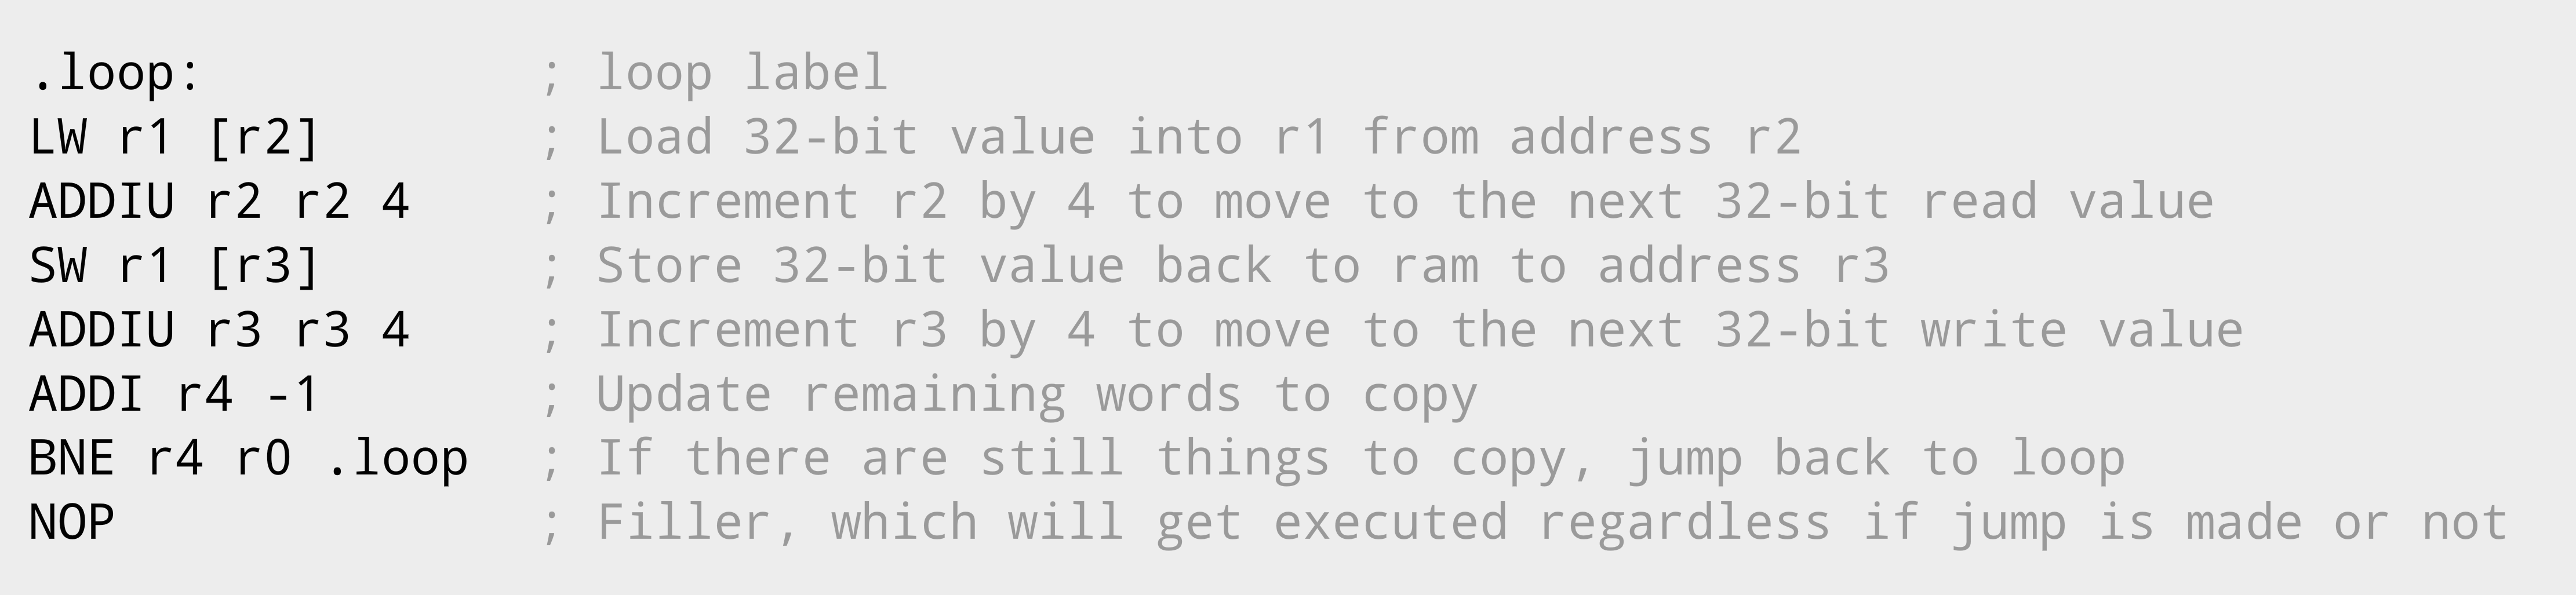
\includegraphics[width=0.8\textwidth]{obrazky-figures/slow-copy.png}
	\caption{Pomocí 7 instrukcí a správným prokládáním lze docílit maximální rychlosti při kopírování dat. Každý cyklus přenese 4 byty.}
	\label{slow-copy}
\end{figure}

Z teoretického hlediska to znamená, že rychlost přenosu činí $\frac{33.8688}{4+3}\times4 = 19.3536 MB/s$. 
Kvůli této nevýhodě obsahuje \textit{PlayStation} komponentu \textit{Direct Memory Access (DMA)}, 
která slouží výhradně k~velmi rychlému přenosu dat mezi pamětí \textit{RAM} a hardwarovými komponentami. 
\textit{DMA} má celkem 7 různých kanálů, přičemž každý kanál specifikuje komunikující komponenty\footnote{DMA\cite{PSXSpec} \url{https://psx-spx.consoledev.net/dmachannels/}}.

\begin{itemize}
    \item{\textbf{0 - MDECIN} - Z \textit{RAM} do \textit{MDEC} vstupu}
    \item{\textbf{1 - MDECOUT} - Z \textit{MDEC} výstupu do \textit{RAM}}
    \item{\textbf{2 - GPU} - Mezi \textit{RAM} a \textit{GPU}}
    \item{\textbf{3 - CDROM} - Z \textit{CD-ROM} do \textit{RAM}}
    \item{\textbf{4 - SPU} - Mezi \textit{RAM} a \textit{SPU}}
    \item{\textbf{5 - PIO} - Mezi \textit{RAM} a \textit{Expansion Port}}
    \item{\textbf{6 - OTC} - Mezi \textit{RAM} a \textit{GPU Ordering Table}}
\end{itemize}

\textit{DMA} také poskytuje celkem 3 různé módy přenosu:

\begin{itemize}
    \item{\textbf{Word Copy} - Jde o rychlý přenos lineární sekvence 32-bitových hodnot. Maximálně se může přenést až \textit{65536} 32-bitových hodnot.}
    \item{\textbf{Block Copy} - Přenáší se bloky o uživatelem definované délce. Provedení přenosu také závisí na připravenosti komponenty.}
    \item{\textbf{Linked List Copy} - Přenášená data se dělí na hlavičku a tělo. Hlavička obsahuje délku těla a adresu další hlavičky. Celá datová struktura je pak řetězec hlaviček a těl.}
\end{itemize}

Každý mód přenosu poskytuje velmi rychlé přenosy, protože \textit{DMA} využívá \textit{DRAM Hyper Page} mód, 
což umožňuje \textit{DMA} přistupovat k \textit{DRAM} řádkům v jednom procesorovém cyklu. 
Tento přístup má minimální režii, která způsobí, že pro každých 17 cyklů se přečte 16 32-bitových slov.

Při \textit{DMA} přenosu má \textit{CPU} přísná pravidla ohledně přístupu do paměti. 
Pokud probíhá přenos, \textit{CPU} může přistupovat k vyrovnávacím pamětem a ke svým dvěma koprocesorům. 
Jakmile se \textit{CPU} pokusí přistoupit do paměti, je jeho chod pozastaven, dokud \textit{DMA} přenos není dokončen.

Díky tomuto faktu lze v emulátoru jakoukoliv \textit{DMA} synchronizaci obejít tím, že celý přenos se provede najednou a \textit{CPU} je pozastaveno. 
Výjimkou je \textit{MDEC}, kde tato komponenta indikuje připravenost přenosu dat.

\section{Ovladač přerušení/výjimek}

Aby \textit{CPU} mělo přehled o různých událostech, jako je například dokončení \textit{DMA} přenosu, 
\textit{PlayStation} má 2 úzce svázané hardwarové komponenty: \textit{Ovladač přerušení} a \textit{Ovladač výjimek}. 
\textit{Ovladač přerušení} je propojen v podstatě se všemi ostatními komponentami, od kterých je schopen přijímat požadavky na přerušení. 
Tento čip také obsahuje stavový registr, u kterého lze zjistit, kdo přerušení způsobil.

To ale není dostatečné pro pozastavení chodu procesoru. 
\textit{Ovladač přerušení} je napojen na \textit{koprocesor 0 CPU}, tedy \textit{Ovladač výjimek}, 
přičemž přerušení je pouze zvláštní typ výjimky.

\textit{BIOS} následně disponuje předem definovanými vektory adres, na jejichž základě se rozhoduje, 
kam předelegovat řízení procesoru a následně zpracovat výjimku.

\section{Časovače}

\textit{PlayStation} má 3 různé druhy časových zdrojů, plus jeden časový zdroj pro \textit{CPU}. 
Jelikož se tyto 3 hardwarové složky příliš neliší, využil jsem \textit{STL} knihovnu \textit{C++} k instanciaci každého ze tří zdrojů.

\textit{První} zdroj se nazývá \textbf{Dot Clock}. Tento zdroj souvisí s renderovacím módem \textit{GPU} komponenty. 
\textit{Dot} v tomto kontextu reprezentuje jeden vykreslený fragment (tzn. ne pixel na obrazovce. Fragment může mít větší či menší velikost než pixel.) a tento 
zdroj tedy počítá počet vykreslených fragmentů, přičemž rychlost závisí na vertikálním rozlišení \textit{GPU}.

\textit{Druhý} zdroj také souvisí s \textit{GPU} a jeho název je \textbf{Horizontal Blank Clock}. 
Pokaždé, když \textit{GPU} dokončí kreslení jednoho řádku \textit{Framebufferu}, tento zdroj je inkrementován o jedničku. 
Rychlost závisí na regionu konzole a verzi \textit{BIOSu} (\textit{NTSC}/\textit{PAL}).

\textit{Třetí} zdroj je \textbf{System Clock}, který odráží zdroj hodin \textit{CPU}, ale je o osminu zpomalený.

Každý z těchto časovačů má také schopnost vyvolat přerušení, pokud dosáhne určité hodnoty. 
Všechny tyto časovače, kromě svých specifických zdrojů, mají také zdroj hodin \textit{CPU} a jsou schopny svůj zdroj měnit\footnote{Časovače\cite{PSXSpec} \url{https://psx-spx.consoledev.net/timers/}}.

\section{MDEC}

Tento hardwarový čip je jedním z hlavních komponent, která učinila \textit{PlayStation} velmi populární konzolí.
Jelikož se \textit{Sony} rozhodlo použít \textit{CD} jako hlavní úložiště pro hry, každá hra měla v té době
velký prostor. V porovnání se svým konkurentem, \textit{Nintendo 64}, který mohl ukládat maximálně \textit{64 MB},
\textit{PlayStation} disponoval až \textit{600 MB}, přičemž hra mohla obsahovat i více disků a hráč mohl během hry
měnit disky podle postupu ve hře.

Takový prostor bylo třeba využít a \textit{Sony} se rozhodlo pro video. \textit{MDEC} je čip speciálně věnovaný
dekódování speciálního formátu videa. Hlavní myšlenkou tohoto formátu byl \textit{JPEG}. \textit{JPEG} používá
několik kompresních technik, které efektivně kombinuje dohromady. Obrázek je rozdělen na \textit{makrobloky} o velikosti
8x8 nebo 16x16 pixelů. Tyto bloky jsou následně převedeny do \textit{YCbCr} barevného formátu a \textit{CbCr} složky jsou
zploštěny na polovinu. Toto je možné, protože lidské oko je citlivější na intenzitu světla než na samotnou diferenci barev.
Poté je provedena \textit{Discrete Cosine Transform (DCT)}, frekvenční analýza a přebytečné frekvence jsou odstraněny
pomocí kvantizační tabulky. Výsledný makroblok je přeorganizován \textit{Zig Zag} vzorem a zakódován pomocí \textit{Run-Length}
kódování. \textit{JPEG} pak využívá \textit{Huffmanova} kódování pro vytvoření výsledného datového toku.
Dekódování probíhá velmi podobným způsobem, ale obráceným směrem\footnote{MDEC\cite{PSXSpec} \url{https://psx-spx.consoledev.net/macroblockdecodermdec/}}.

Formát snímku videa v \textit{PlayStationu} je velice podobný \textit{JPEGu}, s výjimkou toho, že \textit{PlayStation} nepoužívá \textit{Huffmanovo} kódování.

\begin{figure}[hbt]
	\centering
	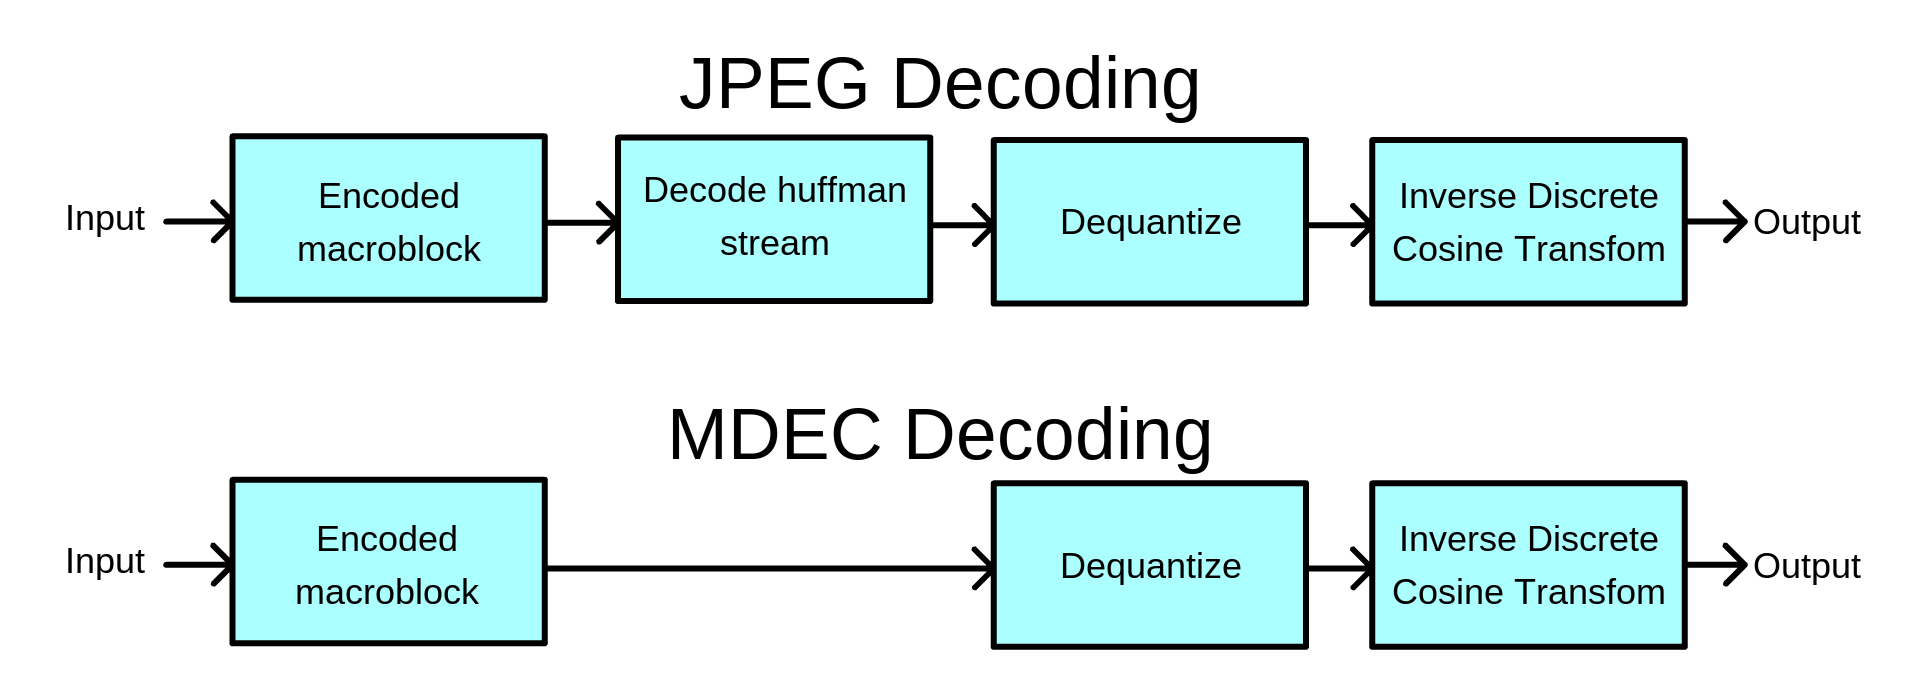
\includegraphics[width=0.8\textwidth]{obrazky-figures/mdec-decoding.png}
	\caption{\textit{MDEC} má velmi podobnou strukturu jako \textit{JPEG} až na vynechaný krok Huffmanova dekódování.}
	\label{mdec-decoding}
\end{figure}

Při přesunu dat, \textit{MDEC} má speciální příznak pomocí kterého indikuje stav dekódování (připravenost vstupu a výstupu).

\section{CD-ROM mechanika}

\textit{Sony} se rozhodlo použít pro herní úložiště \textit{Compact Disc Extended Architecture (CD-XA)} a standard ISO 9660.
\textit{BIOS} se stará o analýzu ISO 9660 souborového systému, \textit{PlayStation} obsahuje speciální \textit{CD-ROM} mechaniku
pro čtení \textit{CD}.

\textit{CPU} může komunikovat s \textit{CD-ROM} mechanikou jednak přes registry a příkazy, ale \textit{CD-ROM} má také tři datové fronty,
pomocí nichž se přenášejí data a dotazy na přerušení. Interně \textit{CD-ROM} disponuje celkem \textit{37} příkazy, pomocí kterých
lze manipulovat s čtecím motorem.

Pro správný přístup k \textit{CD} je nutné správně adresovat toto médium. Jelikož je \textit{CD-ROM} spíše chápán jako
uložiště pro audio či video média, disk je adresován pomocí stop. Každá stopa se dá reprezentovat indexem
nebo formátem \textit{minuty (MM):sekundy (SS):zlomky (FF)}. Každý disk má maximálně \textit{74} minut, přičemž v každé minutě
je \textit{60} sekund a každá sekunda obsahuje \textit{75} zlomků. S touto znalostí se pak tento 
formát dá převést na \textit{Logical Block Addressing (LBA)}, což je schopnost adresovat \textit{CD} jako lineární paměť bytů.

Hry také měly možnost být prodávány ne na jednom, ale na několika discích. \textit{CD-ROM} má pak schopnost výměny disku
bez resetu konzole. Pomocí vypnutí motoru lze \textit{CD-ROM} mechaniku pozastavit, otevřít poklop, vyměnit disk
a program po uzavření poklopu může bezproblémově pokračovat\footnote{CD-ROM mechanika\cite{PSXSpec} \url{https://psx-spx.consoledev.net/cdromdrive/}}.

\section{Periférie}

Ačkoliv samotná konzole má vnitřně několik typů periférií, jako jsou I/O a debugovací porty, veřejně dostupná verze konzole má celkem 4 porty, 
se kterými běžný uživatel může interagovat. Z těchto portů slouží 2 na vsunutí \textit{MemoryCard}, 
což figurovalo jako malé uložiště pro uchování postupu ve hrách. 
Zbývající 2 porty pak fungují jako vstupy pro herní ovladače, kde existují celkem 3 podporované typy: \textit{Digital}, \textit{Analog} a \textit{Mouse}. 
Nicméně drtivá většina celé \textit{PlayStation} knihovny používá pouze \textit{Digital} verzi ovladače.

Hry mohou individuálně číst z těchto portů a umožňují tak uživateli s konzolí interagovat. 
Veškerá komunikace mezi \textit{CPU} a perifériemi probíhá pomocí \textit{Serial I/O (SIO)}\footnote{Ovladače a paměťové karty\cite{PSXSpec} \url{https://psx-spx.consoledev.net/controllersandmemorycards/}}.













